\documentclass{article}
\usepackage[margin=1.5cm,bottom=2cm]{geometry}
\usepackage{fancyhdr}
\usepackage{graphicx}
\pagestyle{fancy}
\usepackage{enumitem,amssymb}
\newlist{todolist}{itemize}{2}
\setlist[todolist]{label=$\square$}

\begin{document}
\fancyhead[L]{ 
\includegraphics[width=2cm]{au_logo.png} }
\fancyhead[R]{PHYS 2250: General Physics II}
\fancyfoot[C]{\thepage}
\vspace*{0cm}
\begin{center}
	{\LARGE \textbf{Quiz 3}}
	%\vspace{0.25cm}
	%{\Large Due: Friday, September 11}
\end{center}

\begin{enumerate}
	\item Consider a uniformly charged rod of length $L$ carrying a total charge $Q$. The rod is oriented on the positive $y$ axis, with one end at the origin. Write an expression for the electric field due to the rod at a distance $x$ along the $x$ axis. You may leave your expression in integral form.
	
	\begin{figure}[ht!]
		\centering
		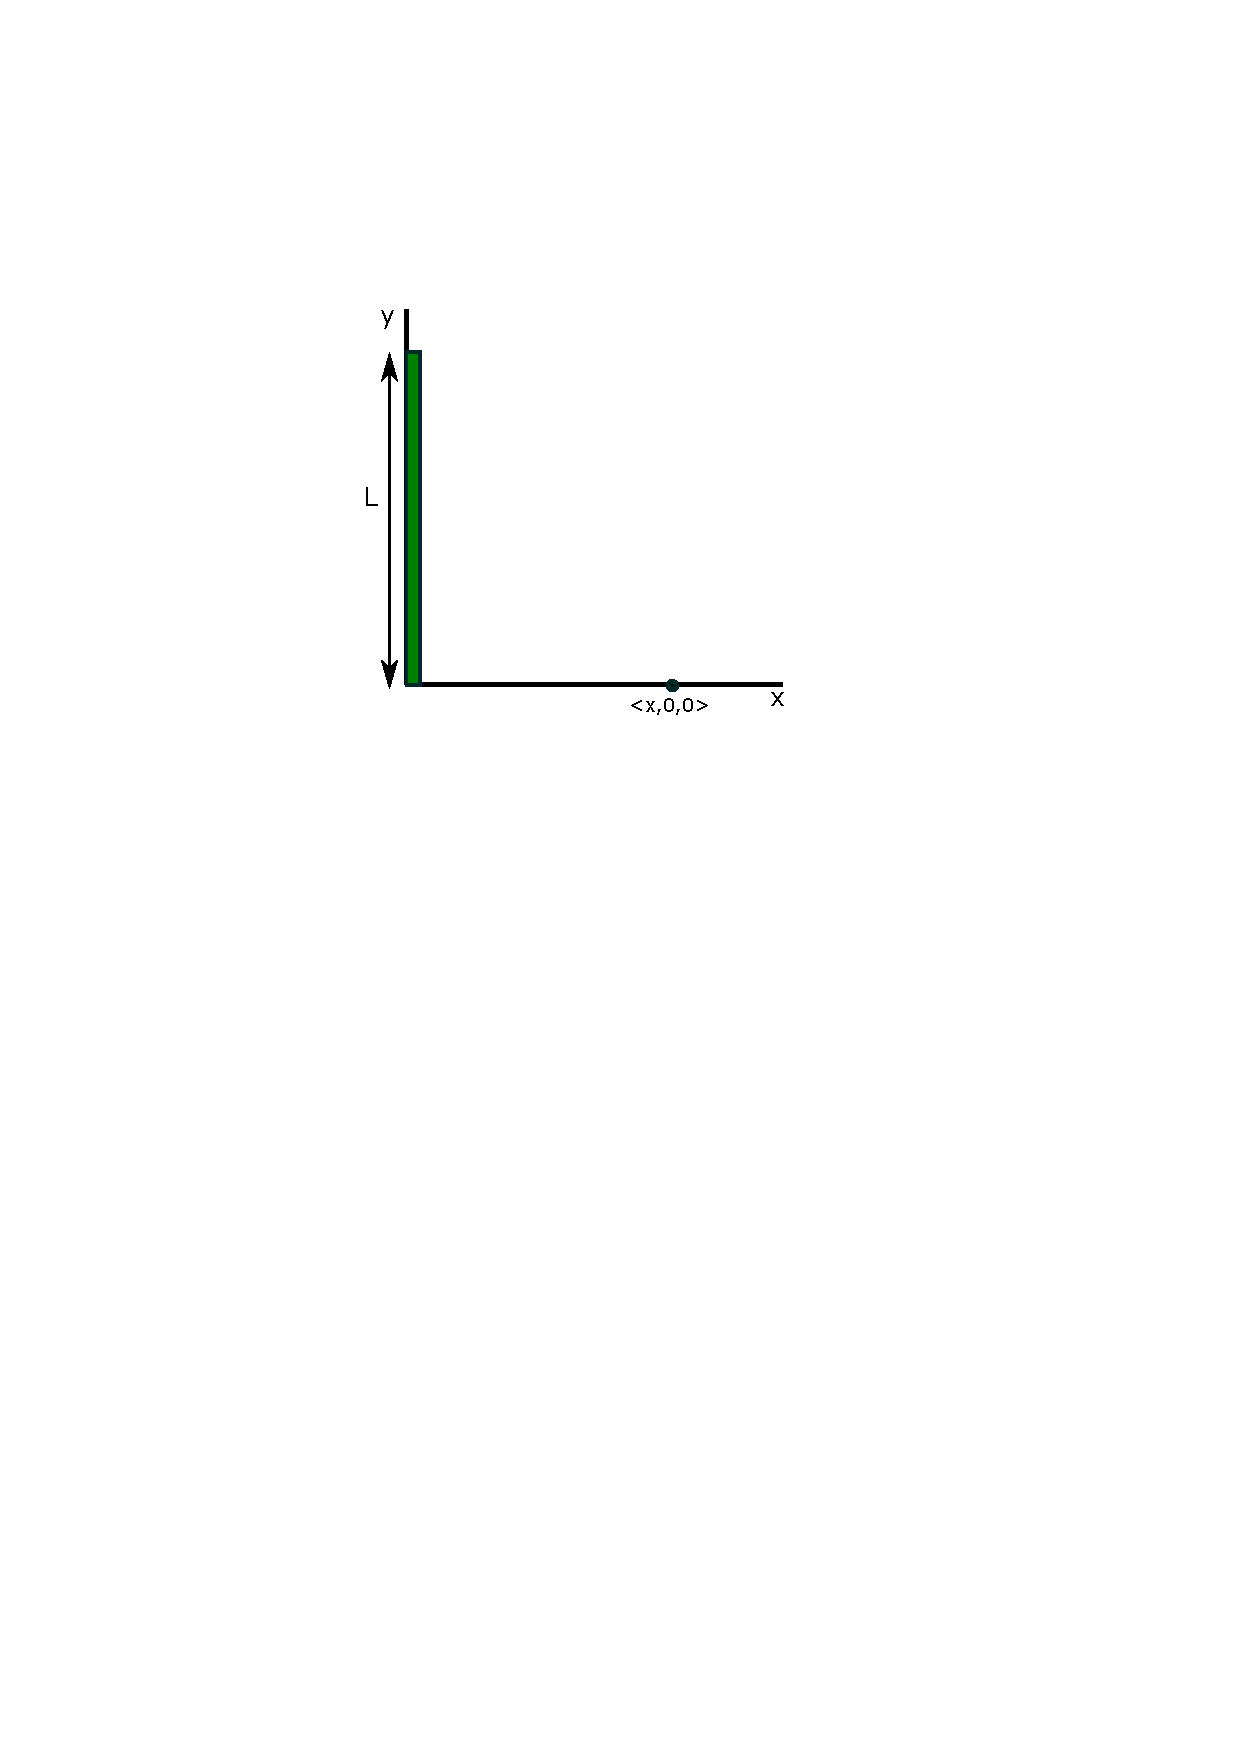
\includegraphics[width=6cm]{charged_rod.pdf}
	\end{figure}
\end{enumerate}

\end{document}